\begin{figure}[H]
	\centering
	\subfloat[]{
		\resizebox{0.65\textwidth}{!}{
			      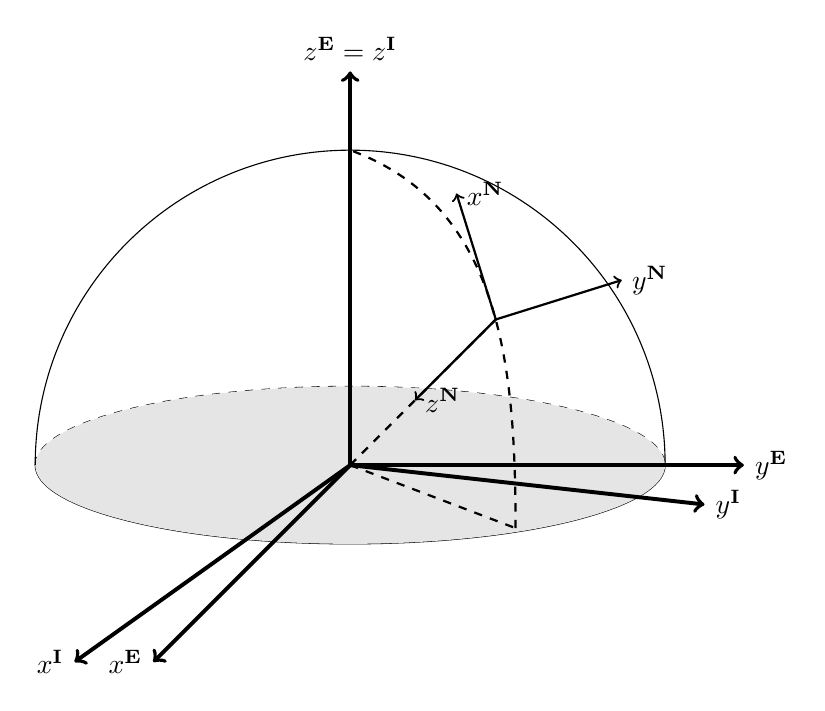
\begin{tikzpicture}
			        % base circle
			        \draw (-4,0) arc (180:360:4 and 1);
			        \draw [dashed] (-4,0) arc (180:0:4 and 1);

			        % fill
			        \filldraw[fill=gray!20, draw=none] (-4,0) arc (180:360:4 and 1) -- (4,0) arc (0:180:4 and 1) -- cycle;


			        % Circle around the plate border
			        \draw (-4,0) arc (180:0:4 and 4);


			        % Draw the lines
			        \draw [thick, ->, line width=.5mm] (0,0) -- ++(-2.5,-2.5) node [left] {$x^{\mathbf{E}}$};
					\draw [thick, ->, line width=.5mm] (0,0) -- ++(-2.5-1,-2.5) node [left] {$x^{\mathbf{I}}$};
			        \draw [thick, ->, line width=.5mm] (0,0) -- ++(0,5) node [above] {$z^{\mathbf{E}}=z^{\mathbf{I}}$};
			        \draw [thick, ->, line width=.5mm] (0,0) -- ++ (5,0) node [right] {$y^{\mathbf{E}}$};
					\draw [thick, ->, line width=.5mm] (0,0) -- ++ (4.5,-0.5) node [right] {$y^{\mathbf{I}}$};


			        % define coordinate
			        \coordinate (A) at (2.1,-.8);
			        % Draw the dashed line from center to plate border
			        \draw [thick, dashed] (0,0) -- ++ (A);

			        % Draw the arc from the top of the circle to the dashed line
			        % \tikz[every to/.style={bend left}]
			        \draw [thick, dashed] (2.1,-.8) to
			        [out=90,in=-20]
			        (0,4);


			        \coordinate (B) at (1.85,1.85);

			        \draw [thick, dashed] (0,0) -- ++ (B);

			        % Navigation coordinate system
			        % x axis
			        \draw [thick, ->] (B) -- ++ (-.5, 1.6) node [right] {$x^{\mathbf{N}}$};
			        % y axis
			        \draw [thick, ->] (B) -- ++ (1.6, .5) node [right] {$y^{\mathbf{N}}$};
			        % z axis
			        \draw [thick, ->] (B) -- ++ (-1.85/1.8, -1.85/1.8) node [right] {$z^{\mathbf{N}}$};
			    \end{tikzpicture}
			      }\label{fig:navigation}}
	\\
	\hspace{-3cm}
	\subfloat[]{
		\resizebox{.8\textwidth}{!}{
    \begin{tikzpicture}
        % Add horizontal space before the image to shift it to the right
         % Adjust this value to move the image horizontally
        \begin{scope}
            \node[anchor=south west,inner sep=0] (image) at (0,0) {\includegraphics[width=1.5\textwidth]{../Figure/ship.png}};
            \begin{scope}[x={(image.south east)},y={(image.north west)}]
            % add center of mass
            \node at (image.center) {\centerofmass};
            % add x axis
            \draw[->, line width=0.5mm] (image.center) -- ++(0.5,-0.22) node [right] {\Huge $x^{\mathbf{M}}$};
            % add y axis
            \draw[->, line width=0.5mm] (image.center) -- ++(-0.3,-0.3) node [below] {\Huge $y^{\mathbf{M}}$};
            % add z axis
            \draw[->, line width=0.5mm] (image.center) -- ++(0,-0.4) node [below] {\Huge $z^{\mathbf{M}}$};
            \end{scope}
        \end{scope}
    \end{tikzpicture}%
}\label{fig:master}}
	\hspace{-1cm}
	\subfloat[]{
		% \hspace{-4cm}
		\resizebox{0.3\textwidth}{!}{
		\begin{tikzpicture}
	        \begin{scope}
	            \node[anchor=south west,inner sep=0] (image) at (0,0) {\includegraphics[width=0.7\textwidth]{../Figure/otter.png}};
	            \begin{scope}[x={(image.south east)},y={(image.north west)}]
	            % add center of mass
	            \node at (image.center) {\centerofmass};
	            % add x axis
	            \draw[->, line width=0.5mm] (image.center) -- ++
	            (0.5,-0.07) node [right] {\Huge $x^{\mathbf{S}}$};
	            % add y axis
	            \draw[->, line width=0.5mm] (image.center) -- ++
	            (-0.4*1.5,-0.1*1.5) node [below] {\Huge $y^{\mathbf{S}}$};
	            % add z axis
	            \draw[->, line width=0.5mm] (image.center) -- ++
	            (0,-0.4) node [below] {\Huge $z^{\mathbf{S}}$};
	            % center of mass text
	            % \node at (image.center) [
	            % yshift=1.5cm, xshift=1.5cm]
	            % {Center of Mass};
	            \end{scope}
	        \end{scope}
	    \end{tikzpicture}%
		}\label{fig:slave_otter}}

	\caption{Graphical Representation of the Presented Reference Frames:~\ref{sub@fig:navigation} Inertial, Earth, and Navigation Frames~\ref{sub@fig:master}~Master Frame~\ref{sub@fig:slave_otter} Slave Frame
	}\label{fig:frames}
\end{figure}
